% ----------------------------------------------------------------- %
%             The Speech Signal Processing Toolkit (SPTK)           %
%             developed by SPTK Working Group                       %
%             http://sp-tk.sourceforge.net/                         %
% ----------------------------------------------------------------- %
%                                                                   %
%  Copyright (c) 1984-2007  Tokyo Institute of Technology           %
%                           Interdisciplinary Graduate School of    %
%                           Science and Engineering                 %
%                                                                   %
%                1996-2017  Nagoya Institute of Technology          %
%                           Department of Computer Science          %
%                                                                   %
% All rights reserved.                                              %
%                                                                   %
% Redistribution and use in source and binary forms, with or        %
% without modification, are permitted provided that the following   %
% conditions are met:                                               %
%                                                                   %
% - Redistributions of source code must retain the above copyright  %
%   notice, this list of conditions and the following disclaimer.   %
% - Redistributions in binary form must reproduce the above         %
%   copyright notice, this list of conditions and the following     %
%   disclaimer in the documentation and/or other materials provided %
%   with the distribution.                                          %
% - Neither the name of the SPTK working group nor the names of its %
%   contributors may be used to endorse or promote products derived %
%   from this software without specific prior written permission.   %
%                                                                   %
% THIS SOFTWARE IS PROVIDED BY THE COPYRIGHT HOLDERS AND            %
% CONTRIBUTORS "AS IS" AND ANY EXPRESS OR IMPLIED WARRANTIES,       %
% INCLUDING, BUT NOT LIMITED TO, THE IMPLIED WARRANTIES OF          %
% MERCHANTABILITY AND FITNESS FOR A PARTICULAR PURPOSE ARE          %
% DISCLAIMED. IN NO EVENT SHALL THE COPYRIGHT OWNER OR CONTRIBUTORS %
% BE LIABLE FOR ANY DIRECT, INDIRECT, INCIDENTAL, SPECIAL,          %
% EXEMPLARY, OR CONSEQUENTIAL DAMAGES (INCLUDING, BUT NOT LIMITED   %
% TO, PROCUREMENT OF SUBSTITUTE GOODS OR SERVICES; LOSS OF USE,     %
% DATA, OR PROFITS; OR BUSINESS INTERRUPTION) HOWEVER CAUSED AND ON %
% ANY THEORY OF LIABILITY, WHETHER IN CONTRACT, STRICT LIABILITY,   %
% OR TORT (INCLUDING NEGLIGENCE OR OTHERWISE) ARISING IN ANY WAY    %
% OUT OF THE USE OF THIS SOFTWARE, EVEN IF ADVISED OF THE           %
% POSSIBILITY OF SUCH DAMAGE.                                       %
% ----------------------------------------------------------------- %
\hypertarget{histogram}{}
\name{histogram}{histogram}{data processing}

\begin{synopsis}
\item [histogram] [ --l $L$ ] [ --i $I$ ] [ --j $J$ ] [ --s $S$ ] [ --n ] 
                  [ {\em infile} ] 
\end{synopsis}

\begin{qsection}{DESCRIPTION}
{\em histogram} makes histograms of frames of input data 
from {\em infile} (or standard input), 
sending the results to standard output.

Input and output data are in float format.
The output can be graphed with \hyperlink{fdrw}{fdrw}.

If an input value is outside the specified interval, 
the exit status of histogram will be nonzero, 
but the output histogram will still be created.
\end{qsection}

\begin{options}
        \argm{l}{L}{frame size\\
          \begin{tabular}{ll}\\ [-1ex]
            $L>0$ & evaluate the histogram for every frame\\
            $L=0$ & evaluate the histogram for the whole file\\
          \end{tabular}\\\hspace*{\fill}}{0}
        \argm{i}{I}{infimum}{0.0}
        \argm{j}{J}{supremum}{1.0}
        \argm{s}{S}{step size}{0.1}
        \argm{n}{}{normalization}{FALSE}
\end{options}

\begin{qsection}{EXAMPLE}
The example below plots the histogram of the speech waveform file
{\em data.f} in float format.
\begin{quote}
 \verb!histogram -i -16000 -j 16000 -s 100 data.f | fdrw | xgr!
\end{quote} 
\begin{center}
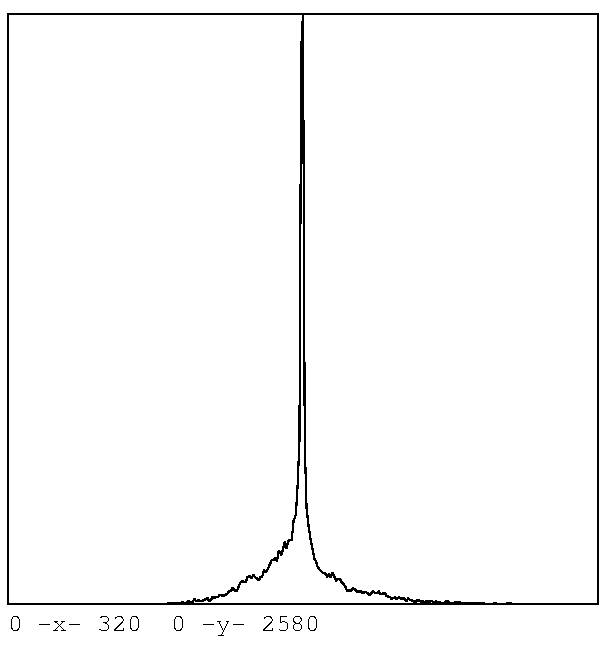
\includegraphics[width=6cm]{fig/histogram.pdf}
\end{center}
\end{qsection}

\begin{qsection}{NOTICE}
If $L > 0$, calculate histogram frame by frame.
\end{qsection}

\begin{qsection}{SEE ALSO}
\hyperlink{average}{average}
\end{qsection}
